\chapter{Annexe technique sur les drones}
\label{chap:annexe1}

\section{Système de drone : Paparazzi}

Un drone est composé de plusieurs pièces assemblées entre elles pour former la structure sur laquelle sont fixés des actionneurs, un autopilote et une charge utile (colis, caméra, capteur, etc.). L'élément central est l'autopilote qui assure la communication entre tous les éléments. Nous pouvons décomposer l'autopilote en deux parties : la partie matérielle et la partie logicielle.

La partie matérielle est constituée d'un circuit imprimé (PCB) sur lequel des composants sont installés pour assurer les tâches relatives au vol. Ainsi, nous pouvons détailler les capteurs embarqués et le microcontrôleur avec l'ensemble de ses ports de communication \ref{sec:capteurs} et \ref{sec:micoctrl}. Et la partie logicielle qui se scinde en deux éléments qui sont : le segment sol et le logiciel embarqué \ref{sec:logiciel}.

 \subsection{Les capteurs d'un autopilote}
 \label{sec:capteurs}
 Un autopilote comporte généralement un accéléromètre, un gyroscope, un magnétomètre et un baromètre.
 
 \paragraph{L'accéléromètre}à trois axes permet de mesurer l'ensemble des forces appliquées sur le véhicule à l'exception du poids. Il est possible d'obtenir la position du drone par double intégration de la mesure de l'accéléromètre. Toutefois, il convient de souligner que la position dérive rapidement en raison des bruits de mesure.

 \paragraph{Le gyroscope}à trois axes permet de mesurer les vitesses de rotation du véhicule. Il est possible d'obtenir l'orientation du drone par intégration de la mesure du gyroscope. Toutefois, comme précédemment, l'orientation dérive rapidement en raison des bruits de mesure.

 \paragraph{Le magnétomètre} à trois axes indique la direction du nord magnétique. Il permet de se diriger par rapport à une référence connue. Le principal inconvénient de ce capteur est sa perturbation par les masses magnétiques environnantes, ainsi que par les champs magnétiques parasites induits par la proximité des moteurs électriques par exemple. Il est donc difficile de les utiliser à l'intérieur d'un bâtiment. L'influence magnétique de l'engin porteur et les perturbations dues à d'éventuels moteurs électriques peuvent être éliminées en qualifiant, de manière statique, les erreurs dues aux masses métalliques du véhicule et aux moteurs électriques (en fonction des tensions et courants d'alimentation).

 \paragraph{Le baromètre}est un capteur d'altitude basée sur la mesure de la pression atmosphérique.

 Il est courant de retrouver plusieurs capteurs dans un même boitier, que l'on nomme centrale inertielle (Inertial Measurement Units, IMU), \nomenclature[]{\(IMU\)}{Centrales inertielles (\textit{Inertial Measurement Units})}. Ces dernières sont composées au minimum d'un accéléromètre 3-axes et d'un gyroscope 3-axes, mais il est courant de les trouver avec un magnétomètre 3-axes. 


 \paragraph{Le GPS}est monté en extérieur de l'autopilote. Ce système de géo-positionnement par satellite (\textit{Global Positioning System}, GPS) \nomenclature[]{\(GPS\)}{Géo-positionnement par satellite (\textit{Global Positioning System})} permet d'obtenir un positionnement absolu du drone. 

 \subsection{Le microcontrôleur d'un autopilote}
 \label{sec:micoctrl}
 Le microcontrôleur (Microcontroller Unit, MCU) \nomenclature[]{\(MCU\)}{Microcontrôleurs (\textit{Microcontroller Unit})} est la pièce maitresse de l'autopilote en ce qu'elle permet d'effectuer l'ensemble des traitements nécessaires à la conduite du vol.

 De plus il possède plusieurs ports de communication pour récupérer les données de capteur ou envoyer des ordres aux actionneurs.


 Nous pouvons citer le dshot qui est un protocole de communication défini entre l'autopilote et l'ESC pour envoyer les commandes des moteurs. Les avancées sur ce protocole ont notamment permis la communication bidirectionnelle, permettant d'obtenir la vitesse des moteurs, leurs consommations.

 \todo{Autre protocole can, serial, I2c }

 \subsection{Évolutions}
 Les nombreux progrès dans les systèmes d'estimation état permettent de connaître précisément l'orientation et la position des drones pour assurer la stabilisation, le guidage et la navigation. Les progrès sont liés à l'amélioration continue des capteurs, notamment des centrales inertielles constituées d'un accéléromètre, d'un gyroscope et d'un magnétomètre.

La Table \ref{tab:autopilote_ev} montre l'évolution des vitesses des microcontrôleurs (Microcontroller Unit, MCU) \nomenclature[]{\(MCU\)}{Microcontrôleurs (\textit{Microcontroller Unit})} embarqués sur les autopilotes et de la réduction du bruit des capteurs inertiels.
\begin{table}[ht]
    \centering
    \begin{tabular}{|c|c|c|c|c|c|}
        \hline
        Type & Date & MCU & Vitesse & Capteur  & Bruit RMS \\
        \hline \hline
        \href{https://wiki.paparazziuav.org/wiki/Apogee/v1.00}{Apogee}  & 2013 & STM32F4 & 168 MHz & MPU-9150 & \begin{tabular}{ccc} Gyro : 0.06 dps \\
        Accel: 4 mg  \end{tabular}  \\
        \hline
        \href{https://wiki.paparazziuav.org/wiki/Chimera/v1.00}{Chimera} & 2016 & STM32F7 & 216 MHz &  MPU-9250 & \begin{tabular}{ccc} Gyro : 0.1  dps \\
        Accel: 8 mg  \end{tabular}\\
        \hline
        \href{https://wiki.paparazziuav.org/wiki/Tawaki/v1.10}{Tawaki 1} &2019 &  STM32F7 & 216 MHz  & ICM-20600 & \begin{tabular}{ccc} Gyro : 0.04 dps \\
        Accel: 1 mg  \end{tabular}\\
        \hline
        \href{https://wiki.paparazziuav.org/wiki/Tawaki/v2.01}{Tawaki 2} &2023 &  STM32H7 & 480 MHz & ICM-42688-P & \begin{tabular}{ccc} Gyro : 0.028 dps \\
        Accel: 0.70 mg  \end{tabular} \\
        \hline
    \end{tabular}
    \caption{Évolution des autopilotes paparazzi sur dix ans.}
    \label{tab:autopilote_ev}
\end{table}

Sur une période de dix ans, nous pouvons observer que les microcontrôleurs ont doublé leur vitesse d'exécution, que les fabricants ont divisé par deux le bruit moyen sur les gyroscopes et par quatre le bruit moyen des accéléromètres.
Ces évolutions continues permettent une amélioration de l'estimation du drone utilisée pour la stabilisation. Il en résulte une stabilité accrue et de nouvelles possibilités pour la commande des drones.

 \subsection{Les logiciels d'un autopilote}
 \label{sec:logiciel}
 Tout le fonctionnement d'un drone repose sur le logiciel qui permet de le faire voler. Il se décompose en deux catégories : la partie sol et la partie embarquée.

 \subsection{Le segment sol}
\todo{remplir}
 \subsection{Le logiciel embarqué}
 Le logiciel embarqué 

 fusion de donnée 
 estimation d'état 

 \begin{figure}[ht!]
    \centerline{
    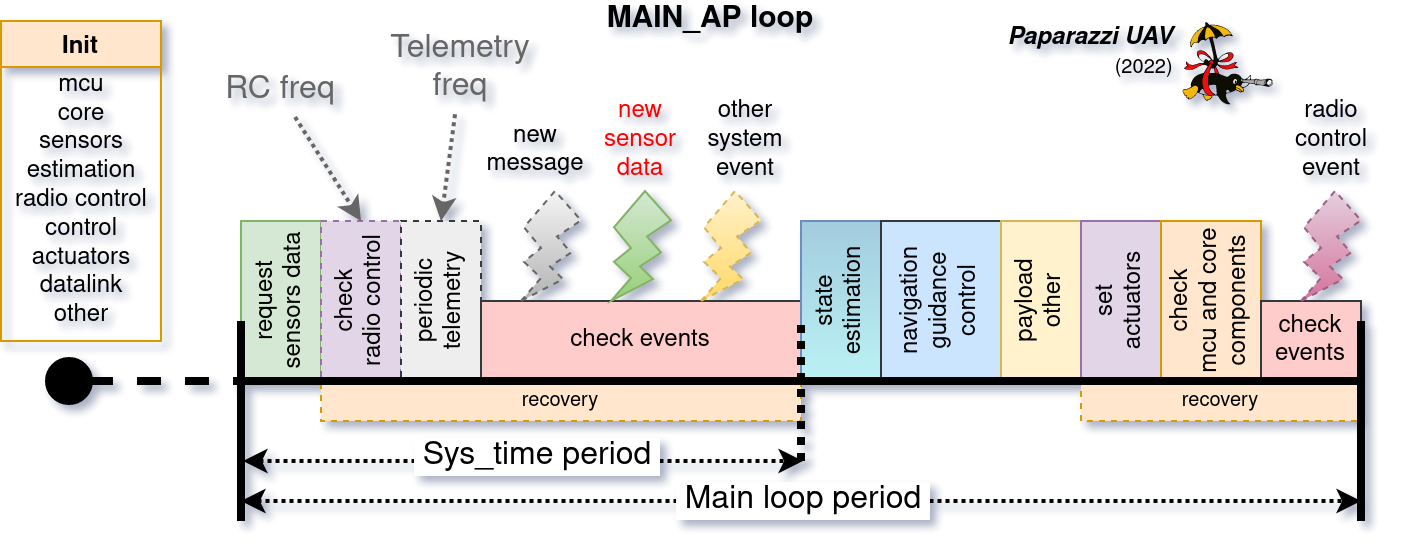
\includegraphics[trim=0cm 0cm 0cm 0cm,clip,width=1\columnwidth]{figures/PPRZ_Main_ap_loop.png}}
    \caption{Todo.}
    \label{fig:schedulingpaparazzi}
\end{figure}


\section{AM32}
\label{sec:AM32}